%%%%%%%%%%%%%%%%%%%%%%%%%%%%%%%%%%%%%%%%%%%%%%%%%%%%%%%%%%%%%%%%%%%%%%%%%%%%%%%%
%2345678901234567890123456789012345678901234567890123456789012345678901234567890
%        1         2         3         4         5         6         7         8

\documentclass[letterpaper, 10 pt, conference]{ieeeconf}

\IEEEoverridecommandlockouts
\overrideIEEEmargins

\usepackage[utf8]{inputenc}
\usepackage[T1]{fontenc}
\usepackage{graphicx}
\usepackage{booktabs}
\usepackage{amsmath}
\usepackage{hyperref}
\usepackage{xcolor}
\usepackage{subcaption}
\usepackage{array}
\setlength{\textfloatsep}{6pt plus 1pt minus 2pt}
\setlength{\floatsep}{4pt plus 1pt minus 2pt}
\setlength{\intextsep}{6pt plus 1pt minus 2pt}
\setlength{\abovecaptionskip}{2pt}
\setlength{\belowcaptionskip}{0pt}
\renewcommand{\topfraction}{0.9}
\renewcommand{\bottomfraction}{0.9}
\renewcommand{\textfraction}{0.05}
\renewcommand{\floatpagefraction}{0.85}
 
\setcounter{topnumber}{3}
\setcounter{bottomnumber}{3}
\setcounter{totalnumber}{6}
\setcounter{dbltopnumber}{2}
\usepackage{placeins}

% Fix for \input in tables with booktabs (LaTeX 2020+ compatibility)
% Source: https://tex.stackexchange.com/questions/611786
\ExplSyntaxOn
\cs_if_exist:NF \expandableinput
  {
    \cs_new:Npn \expandableinput #1
      { \use:c { @@input } { \file_full_name:n {#1} } }
  }
\AddToHook{env/tabular/begin}
  { \cs_set_eq:NN \input \expandableinput }
\ExplSyntaxOff

\title{\LARGE \bf
Online Learning: Randomized Optimization of Neural Network Weights\\
and Gradient-Based Optimizer Analysis
}

\author{siddartha sagar chinne \\
{\tt\small schinne3@gatech.edu}
}

\begin{document}

\maketitle
\thispagestyle{empty}
\pagestyle{empty}

%%%%%%%%%%%%%%%%%%%%%%%%%%%%%%%%%%%%%%%%%%%%%%%%%%%%%%%%%%%%%%%%%%%%%%%%%%%%%%%%
\begin{abstract}
This report investigates four aspects of neural-network online learning on the Adult Income and Wine Quality classification benchmarks: (Part 1) replacing gradient descent with Randomized Optimization (RHC, SA, GA) to tune the output-layer weights; (Part 2) comparing gradient-based optimizer variants (SGD, Nesterov, Adam, AdamW); (Part 3) evaluating regularization techniques (L2, Dropout, Noise, Early Stopping); and (Part 4) a combined gradient + RO fine-tuning strategy. A fixed 60/20/20 train/validation/test split and a 10-seed evaluation protocol are used throughout for fair comparison.
\end{abstract}

%%%%%%%%%%%%%%%%%%%%%%%%%%%%%%%%%%%%%%%%%%%%%%%%%%%%%%%%%%%%%%%%%%%%%%%%%%%%%%%%
\section{INTRODUCTION}

This report continues the analysis from the Supervised Learning (SL) assignment. The best SL checkpoint --- a PyTorch MLP trained on Adam --- serves as the warm-start initialization for all Randomized Optimization experiments in Part 1, grounding RO in a strong local basin. The same two datasets are used: Adult Income (binary classification, 96-dimensional after encoding, 3:1 class imbalance) and Wine Quality (8-class, 11 continuous features, severe class overlap with silhouette score $< 0.1$).

We evaluate four questions: (1) Can derivative-free RO methods match or exceed gradient-based training when restricted to the output layer? (2) How do optimizer variants (SGD, Adam family) differ in convergence speed and final quality? (3) Which regularization strategy best manages the collinearity and overlap identified in EDA? (4) Can chaining gradient + RO fine-tuning outperform either alone?

A key design choice throughout is the use of a fixed 60/20/20 train/validation/test split (rather than the 80/20 + k-fold used in SL). This is required: RO evaluates candidate solutions against the validation set during search, making a held-out validation set mandatory to avoid data leakage.

%%%%%%%%%%%%%%%%%%%%%%%%%%%%%%%%%%%%%%%%%%%%%%%%%%%%%%%%%%%%%%%%%%%%%%%%%%%%%%%%
\section{EXPLORATORY DATA ANALYSIS}

Per the OL assignment guidelines, EDA is summarized briefly here to preserve the same core facts from the SL Report. Preprocessing, leakage controls, and feature decisions are unchanged; any deviations are explicitly disclosed.

\subsection{Adult Income}

The Adult Census dataset~\cite{kohavi1996} contains 45{,}222 samples with 6 numeric and 8 categorical features, expanding to approximately 96 dimensions after one-hot encoding. The class distribution is 3:1 (75.2\% $\leq$50K); we use F1 as the primary metric. A linearity proxy showed only a 1.7\% gap between logistic regression (0.809) and random forest (0.826) under 3-fold CV, confirming the decision boundary is near-linear. Feature--target correlations are weak (max $|r| = 0.24$ for \texttt{age}), and several features are heavily right-skewed.

\textbf{OL implications.} The primary motivation for restricting Randomized Optimization to only the output layer is \emph{computational tractability}: the total parameter space ($\sim$10{,}100 weights) is intractable to search under a 50{,}000-evaluation budget. Restricting to 2 tensors (\texttt{PART1\_RO\_MAX\_TENSORS=2}) limits the search to exactly 202 parameters for Adult and 808 for Wine --- both well below the $\leq$50k cap. Collinear one-hot-encoded features (e.g., \texttt{education} vs.\ \texttt{education-num}) motivate the Part 3 regularization study: both Dropout and L2 are expected to penalize over-reliance on redundant feature groups.

\subsection{Wine Quality}

The combined red/white wine dataset contains 6{,}497 samples with 11 continuous physicochemical features and an 8-class quality target (ratings 3--9). The \texttt{class} column is an exact copy of the target (100\% match rate) and was removed as a leakage control; the \texttt{type} indicator was also removed. The silhouette score on standardized features is $-0.074$, meaning adjacent quality classes overlap more than random. The linearity proxy gives LR $= 0.465$, RF $= 0.490$ --- both well below 50\% Macro-F1 on this 8-class task.

\textbf{OL implications.} The severe class overlap ($\text{silhouette} = -0.074$) shapes the output-layer loss surface in a way that disadvantages single-state perturbation methods. RHC can only move uphill from its current position; SA can accept worse solutions but still explores one state at a time. Neither can simultaneously combine information from multiple regions of an overlapping class landscape. GA's population-based crossover, by contrast, maintains candidate vectors from different quality-rating regions and can recombine partial solutions --- a structural advantage directly predicted by the overlapping-class geometry, which foreshadows why GA outperforms SA on Wine.

\textbf{OL change disclosure.} The SL report used an 80/20 train/test split with k-fold CV. This report uses a 60/20/20 train/validation/test split. The validation split is mandatory for RO and held consistent across Parts 2--4. This reduces the Adult training set from $\sim$36K to $\sim$27K samples (25\% reduction). StandardScaler and one-hot encoders were fit on the training fold only; test-set statistics remained unseen during preprocessing to prevent leakage.


%%%%%%%%%%%%%%%%%%%%%%%%%%%%%%%%%%%%%%%%%%%%%%%%%%%%%%%%%%%%%%%%%%%%%%%%%%%%%%%%
\section{DATASETS AND METHODOLOGY}

\subsection{Datasets}

Both datasets are described in detail in the SL report. Briefly: Adult Income has 45{,}222 samples expanding to 96 dimensions after one-hot encoding, with a 3:1 class imbalance; we use F1 as the primary metric. Wine Quality has 6{,}497 samples with 11 continuous physicochemical features and 8 quality classes; we use Macro-F1. Leakage controls (removing the \texttt{class} duplicate column from Wine) are identical to the SL assignment.

\subsection{Data Split and Reproducibility}

We use a stratified 60/20/20 train/validation/test split (\texttt{random\_state=42}). The validation split is required for Randomized Optimization, which evaluates the objective function on the validation set at each function evaluation. Using k-fold CV instead would either require re-training the network from scratch at each fold (prohibitively expensive under 50{,}000 function evaluation budgets) or introduce data leakage into the search. The same split is used for Parts 2--4 to ensure a fair cross-part comparison.

All experiments use 10 random seeds (42--51). Final metrics are reported as mean and standard deviation across seeds. PyTorch weight initialization uses \texttt{torch.manual\_seed(seed)} and NumPy RNG is seeded identically. As a sanity check, a majority-class baseline (always predict $\leq$50K on Adult) achieves F1$\,=0.0$ by definition, confirming that all reported F1 values reflect genuine learning rather than class imbalance exploitation.

\subsection{Network Architecture}

The shared backbone is a PyTorch MLP with one hidden layer of 100 ReLU units and a softmax output layer. For Adult: input dimension 96, output dimension 2. For Wine: input dimension 11, output dimension 8. All Parts 2--4 share this architecture. Part 1 additionally loads the best SL checkpoint into this backbone before running RO.

\subsection{Part 1: RO Parameter Space}

Randomized Optimization in Part 1 operates on a \emph{flattened} vector of only the final output-layer parameters (weight matrix + bias vector). This is \textbf{intentional}: exposing all $\sim$10{,}000 architecture parameters would make the search dimensionality intractable within a 50{,}000 function evaluation budget. Restricting to 2 tensors (\texttt{PART1\_RO\_MAX\_TENSORS=2}) limits the search to exactly 202 parameters for Adult ($100\times2 + 2$) and 808 for Wine ($100\times8 + 8$), keeping RO tractable.

The hidden layers remain \emph{frozen} at the SL checkpoint values. All perturbations (Gaussian noise with $\sigma = 0.02$) are applied only to the output-layer vector.

%%%%%%%%%%%%%%%%%%%%%%%%%%%%%%%%%%%%%%%%%%%%%%%%%%%%%%%%%%%%%%%%%%%%%%%%%%%%%%%%
\section{HYPOTHESES}

\textbf{Adult hypothesis.} Because Adult is high-dimensional, sparse after one-hot encoding, and close to a near-linear tabular decision problem, I expect full-network adaptive gradient methods (specifically, Adam's per-parameter adaptive learning rates and momentum smoothing via $\beta_1$ and $\beta_2$) to be more effective than output-layer-only Randomized Optimization. Relative to the SL baseline, I expect only modest gains on Adult: Adam-family methods should converge faster than SGD due to adaptive step sizes, while Part~3 regularization (L2 weight decay, Dropout's multiplicative noise) should yield at most small improvements because the backbone is modest and the main difficulty is optimization over many correlated sparse features rather than severe overfitting.

\textbf{Wine hypothesis.} Because Wine is smaller, noisier, multiclass, and has more overlapping class structure, I expect higher variance across seeds and less reliable improvement from optimizer changes alone. Relative to the SL baseline, I do not expect Part~2-style optimizer swaps to deliver large gains on Wine, but I expect output-layer RO (specifically, GA's population-based crossover and SA's stochastic acceptance via the Metropolis criterion) to be more competitive here than on Adult because the SL warm-start may let population-based or stochastic search exploit local non-convex structure that gradient descent alone does not fully capture.

%%%%%%%%%%%%%%%%%%%%%%%%%%%%%%%%%%%%%%%%%%%%%%%%%%%%%%%%%%%%%%%%%%%%%%%%%%%%%%%%
\section{PART 1: RANDOMIZED OPTIMIZATION}

\subsection{Experimental Setup}

Each RO method is given a budget of 50{,}000 function evaluations. The weight-perturbation distribution is Gaussian $\mathcal{N}(0,\, \sigma^2 I)$ with a \emph{constant} step size $\sigma = 0.02$ throughout (no adaptation schedule). This value is calibrated relative to the SL checkpoint weight magnitudes ($\|w\| \approx 0.1$--$0.5$), placing candidate weights within a tight local basin of the pre-trained solution.

\textbf{RHC}: 4 restarts from the warm-start initialization, each perturbed by a single Gaussian draw with $\sigma = 0.02$. Budget split evenly ($\lfloor 50{,}000/4 \rfloor = 12{,}500$ evaluations per restart; full budget consumed). No early-termination plateau rule: each restart runs its full 12{,}500 evaluations regardless of improvement. Step-size schedule: constant (no adaptation). Acceptance rule: improving-or-equal candidate wins.

\textbf{SA}: Exponential cooling, $T_k = T_0 \cdot d^k$ with $T_0 = 10.0$, $d = 0.9998$, calibrated so $T \approx 0.01$ at evaluation 45{,}000 (leaving 10\% of budget in cold exploitation). Step-size schedule: constant $\sigma = 0.02$ (temperature governs acceptance, not step magnitude). Acceptance rule: Metropolis criterion.

\textbf{GA}: Population size 16, elitism 4 (top-4 survivors copied unchanged each generation), crossover: uniform crossover over the flat parameter vector, mutation: Gaussian perturbation $\mathcal{N}(0, 0.02^2)$ applied independently to each weight with rate 0.08. Selection: fitness-proportional selection from the top half of the population. Each generation costs $\text{population\_size}$ function evaluations.

The SL baseline MLP checkpoint (trained with Adam for up to 20 epochs) is loaded before running any RO method. Before each objective function evaluation (i.e., before measuring validation loss on a candidate weight vector), \texttt{model.eval()} is called to disable any stochastic elements; \texttt{model.train()} is restored after evaluation. The Part 1 architecture has no dropout or batch normalization, so this has no practical effect here, but the protocol is applied consistently for correctness.

\subsection{SA Temperature Schedule Calibration}

A critical implementation detail is the SA cooling schedule. The initial implementation used a decay rate of 0.995, which causes the temperature to collapse to $\approx 3.5 \times 10^{-11}$ by evaluation 5{,}000 --- meaning SA was acting as a greedy hill climber for 97\% of its budget. The corrected decay rate $d = 0.9998$ was derived analytically:

\begin{equation}
d = \left(\frac{T_{\text{final}}}{T_0}\right)^{1/N_{\text{target}}} = (0.001)^{1/45000} \approx 0.9998
\end{equation}

This ensures $T$ remains meaningful throughout the search, enabling the expected explore--exploit trade-off.

\subsection{Results}

Table~\ref{tab:part1} summarizes the 10-seed average F1 scores for each RO method compared to the SL baseline.

\begin{table}[!htbp]
    \centering
    \caption{Part 1: RO Test F1 scores vs SL Baseline (10-seed averages).}
    \label{tab:part1}
    \setlength{\tabcolsep}{3pt}
    \begin{tabular}{@{}lcccc@{}}
    \toprule
    & \multicolumn{2}{c}{\textbf{Adult}} & \multicolumn{2}{c}{\textbf{Wine}} \\
    \cmidrule(lr){2-3} \cmidrule(l){4-5}
    Method & F1 & $\sigma$ & Macro-F1 & $\sigma$ \\
    \midrule
    SL Baseline & 0.6817 & --- & 0.3277 & --- \\
RHC & 0.6774 & 0.0020 & 0.3309 & 0.0183 \\
SA & 0.6806 & 0.0022 & 0.3287 & 0.0013 \\
GA & 0.6760 & 0.0008 & 0.3396 & 0.0068 \\
    \bottomrule
    \end{tabular}
\end{table}

\begin{figure}[!htbp]
    \centering
    \begin{subfigure}[t]{0.49\columnwidth}
        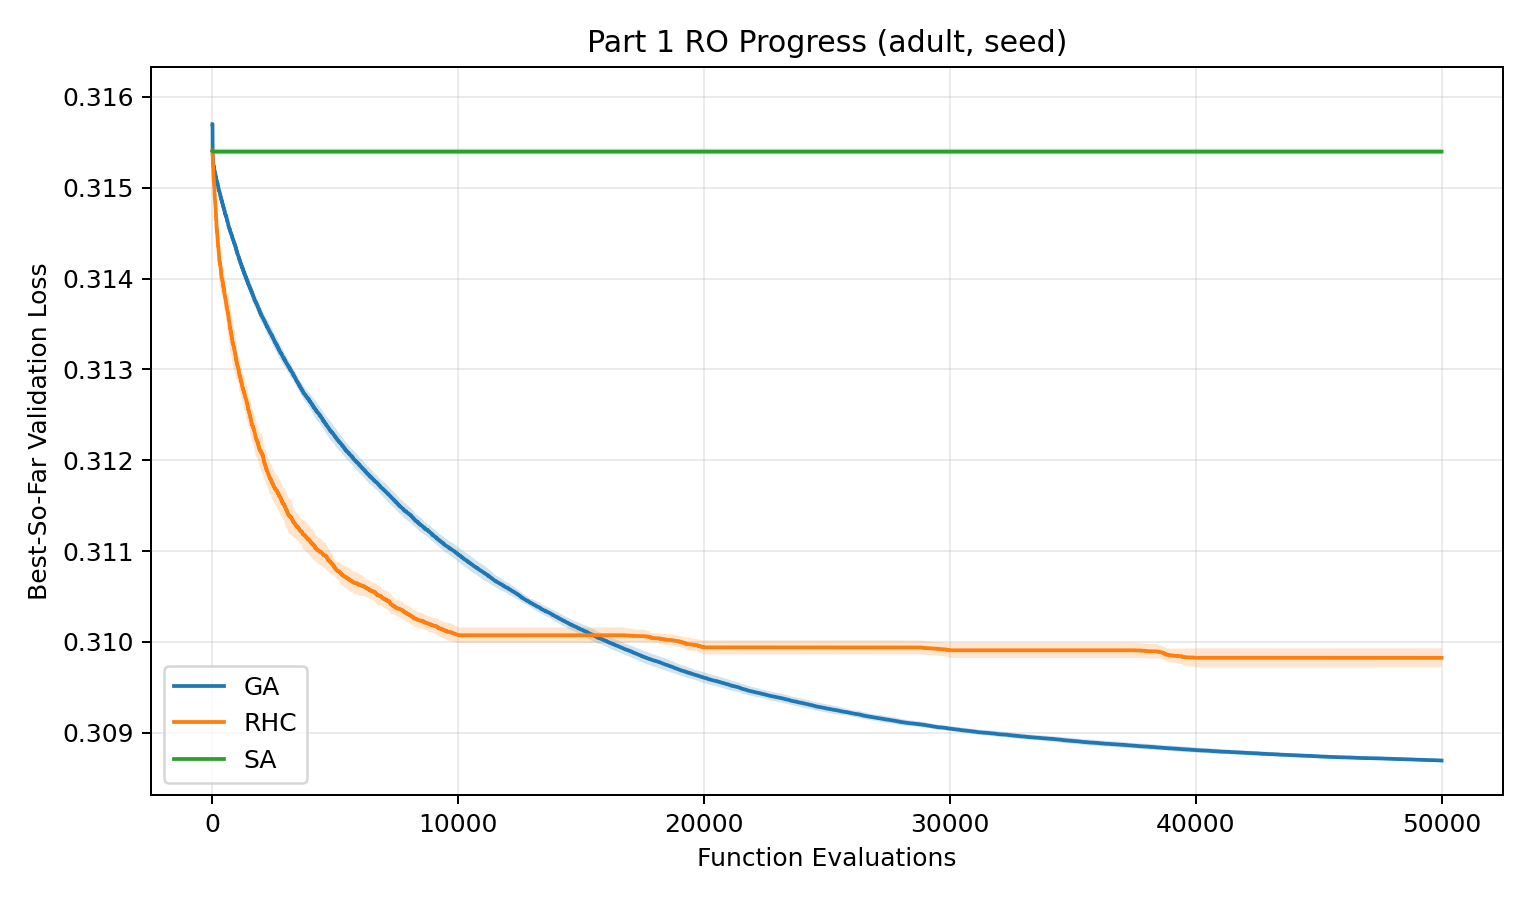
\includegraphics[width=\linewidth]{figures/ro_progress_adult_seed.png}
        \caption{Adult convergence}
    \end{subfigure}
    \hfill
    \begin{subfigure}[t]{0.49\columnwidth}
        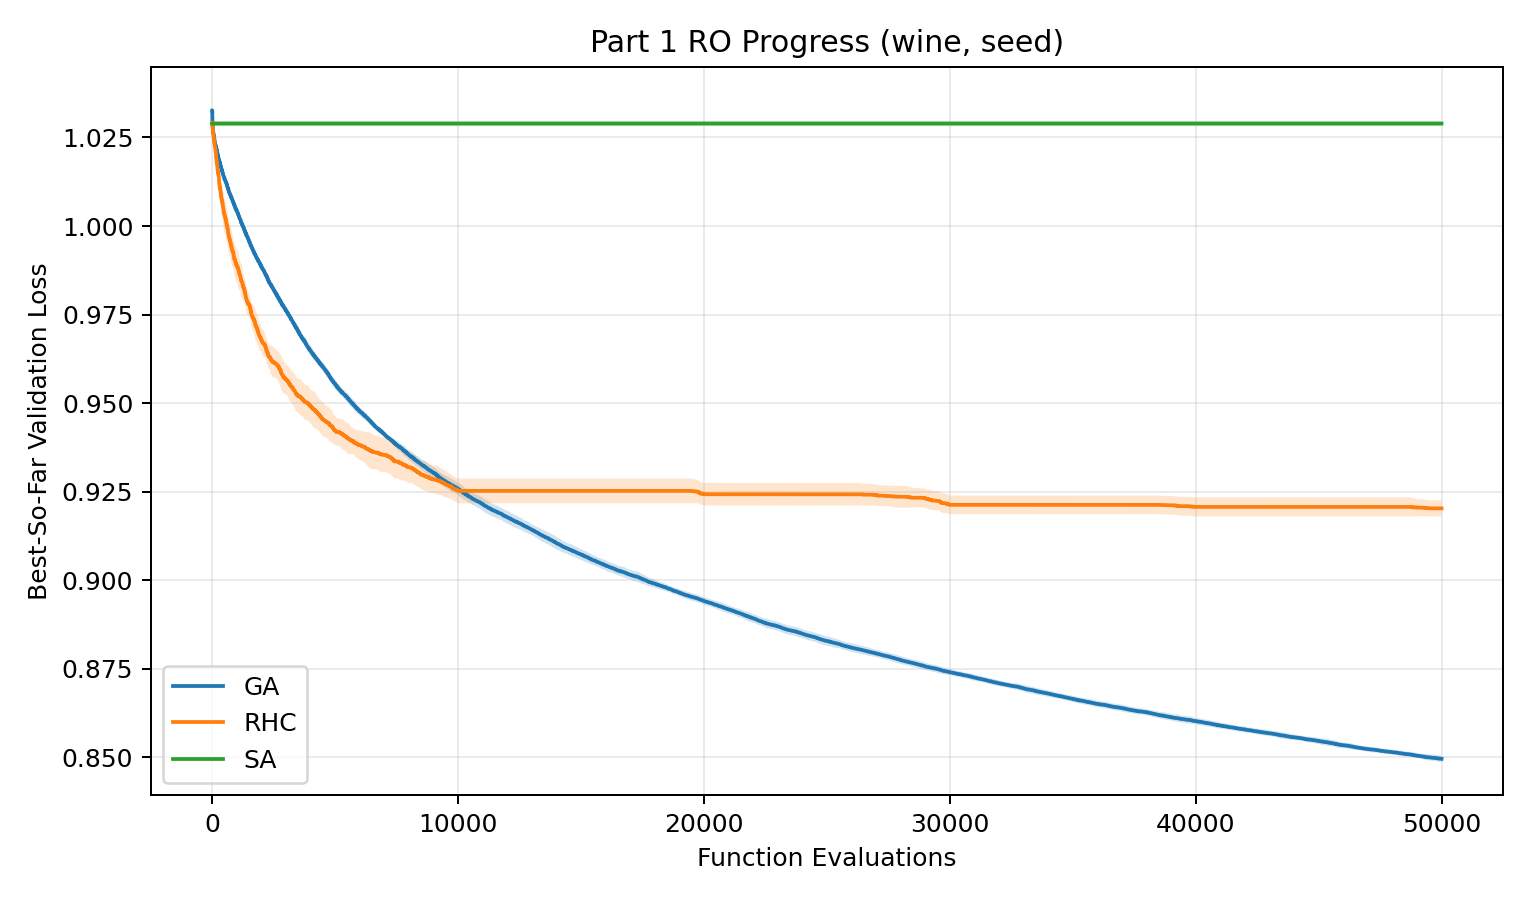
\includegraphics[width=\linewidth]{figures/ro_progress_wine_seed.png}
        \caption{Wine convergence}
    \end{subfigure}
    \caption{Part 1: RO convergence trajectories (val loss vs function evaluations, mean $\pm$ std across 10 seeds). \textbf{Takeaway:} On Adult, GA achieves the lowest val-loss plateau, while SA (green) remains flat --- yet SA achieves the best test F1 (Table~\ref{tab:part1}), suggesting its stochastic acceptance prevents over-optimization to the validation set. On Wine, GA achieves the best final val loss --- confirming the EDA prediction that population-based search advantages single-state methods on overlapping-class loss surfaces.}
    \label{fig:ro_progress}
\end{figure}
\FloatBarrier

\subsection{Hypothesis Validation}

\textbf{The dataset-level hypotheses were partially confirmed.} On Adult, RO did \emph{not} beat the gradient baseline: SA came closest to the SL baseline ($-0.001$ F1) and had narrow variance ($\sigma=0.0022$), but all RO methods remained below the SL result. That is consistent with the expectation that Adult's high-dimensional sparse feature space favors gradient-based optimization over output-layer search. On Wine, however, RO was more competitive than expected: GA outperformed both SA and RHC and exceeded the SL baseline by $+1.2\%$ Macro-F1. This supports the Wine hypothesis that a warm-started population-based search can exploit local non-convex structure in the multiclass output layer more effectively than single-state methods.

%%%%%%%%%%%%%%%%%%%%%%%%%%%%%%%%%%%%%%%%%%%%%%%%%%%%%%%%%%%%%%%%%%%%%%%%%%%%%%%%
\section{PART 2: OPTIMIZER COMPARISON}

\subsection{Experimental Setup}

All Part 2 experiments run on Adult Income only (per assignment scope restrictions). All methods train for up to 20 epochs (approximately 4{,}240 gradient steps on the 60/20/20 split). We define a fixed validation-loss threshold $\ell = 0.32$ for convergence speed analysis. Time and steps to reach $\ell$ are reported as a speed-to-target metric. Methods compared: SGD (no momentum), SGD + Momentum, Nesterov momentum, Adam (baseline), Adam with $\beta_1 = 0$ (RMSProp-like), Adam without bias correction, and AdamW ($\lambda = 10^{-3}$). All use $\text{lr} = 10^{-3}$. The sensitivity heatmaps (Fig.~\ref{fig:part2_sensitivity}) sweep $\alpha \in \{10^{-4}, 5 \times 10^{-4}, 10^{-3}, 2 \times 10^{-3}\}$ and $\beta_1 \in \{0.0, 0.5, 0.9, 0.95\}$ / $\beta_2 \in \{0.9, 0.99, 0.999, 0.9999\}$ for the Adam baseline variant, measuring validation loss after 12 epochs. Typical wall-clock time per method is $\sim$2\,s on a macOS arm64 system (10-core CPU, no GPU).

\subsection{Results}

Table~\ref{tab:part2} shows the Adult F1 and convergence statistics (all 10-seed averages). The Adam baseline reaches a training F1 of $\approx 0.696$ vs.\ a validation F1 of $0.678$, a generalization gap of $\approx 0.018$. SGD shows the largest gap (training $\approx 0.710$, val $0.669$, gap $\approx 0.041$), confirming that without momentum or adaptive rates, the model overfits more within the fixed budget. Adam variants (AdamW, no-BC, $\beta_1{=}0$) all show gaps of $0.018$--$0.020$, nearly identical to the Adam baseline, indicating generalization is bounded by architecture capacity rather than optimizer choice. Interestingly, Adam without bias correction reaches the threshold slightly faster than the baseline ($\sim$212 vs $\sim$424 steps), likely because the underscaled moment estimates in early iterations act as implicit regularization, preventing the optimizer from committing too aggressively to noisy early gradients on this tabular task.

\begin{table}[!htbp]
    \centering
    \caption{Part 2: Optimizer comparison on Adult (10-seed averages). $\ell = 0.32$ val-loss threshold. Steps to $\ell$ are actual values from threshold analysis. Wall-clock on macOS arm64 CPU.}
    \label{tab:part2}
    \setlength{\tabcolsep}{1.5pt}
    \begin{tabular}{@{}lccccc@{}}
    \toprule
    Optimizer & F1 & $\sigma$ & Time to $\ell$ & Steps to $\ell$ & $\Delta$ SL \\
    \midrule
    SL Baseline (Adam) & 0.6817 & --- & $<$1\,s & $<$400 & --- \\
Adam (baseline) & 0.6783 & 0.0043 & $\sim$0.2\,s & $\sim$424 & $-0.0034$ \\
AdamW & 0.6783 & 0.0042 & $\sim$0.2\,s & $\sim$424 & $-0.0034$ \\
Adam (no BC) & 0.6771 & 0.0037 & $\sim$0.1\,s & $\sim$212 & $-0.0045$ \\
Adam ($\beta_1=0$) & 0.6769 & 0.0083 & $\sim$0.3\,s & $\sim$530 & $-0.0047$ \\
SGD + Momentum & 0.6756 & 0.0054 & $\sim$0.3\,s & $\sim$636 & $-0.0061$ \\
Nesterov & 0.6733 & 0.0061 & $\sim$0.3\,s & $\sim$530 & $-0.0084$ \\
SGD & 0.6693 & 0.0044 & $\sim$1.8\,s & $\sim$3{,}816 & $-0.0124$ \\
    \bottomrule
    \end{tabular}
\end{table}

\begin{figure}[!htbp]
    \centering
    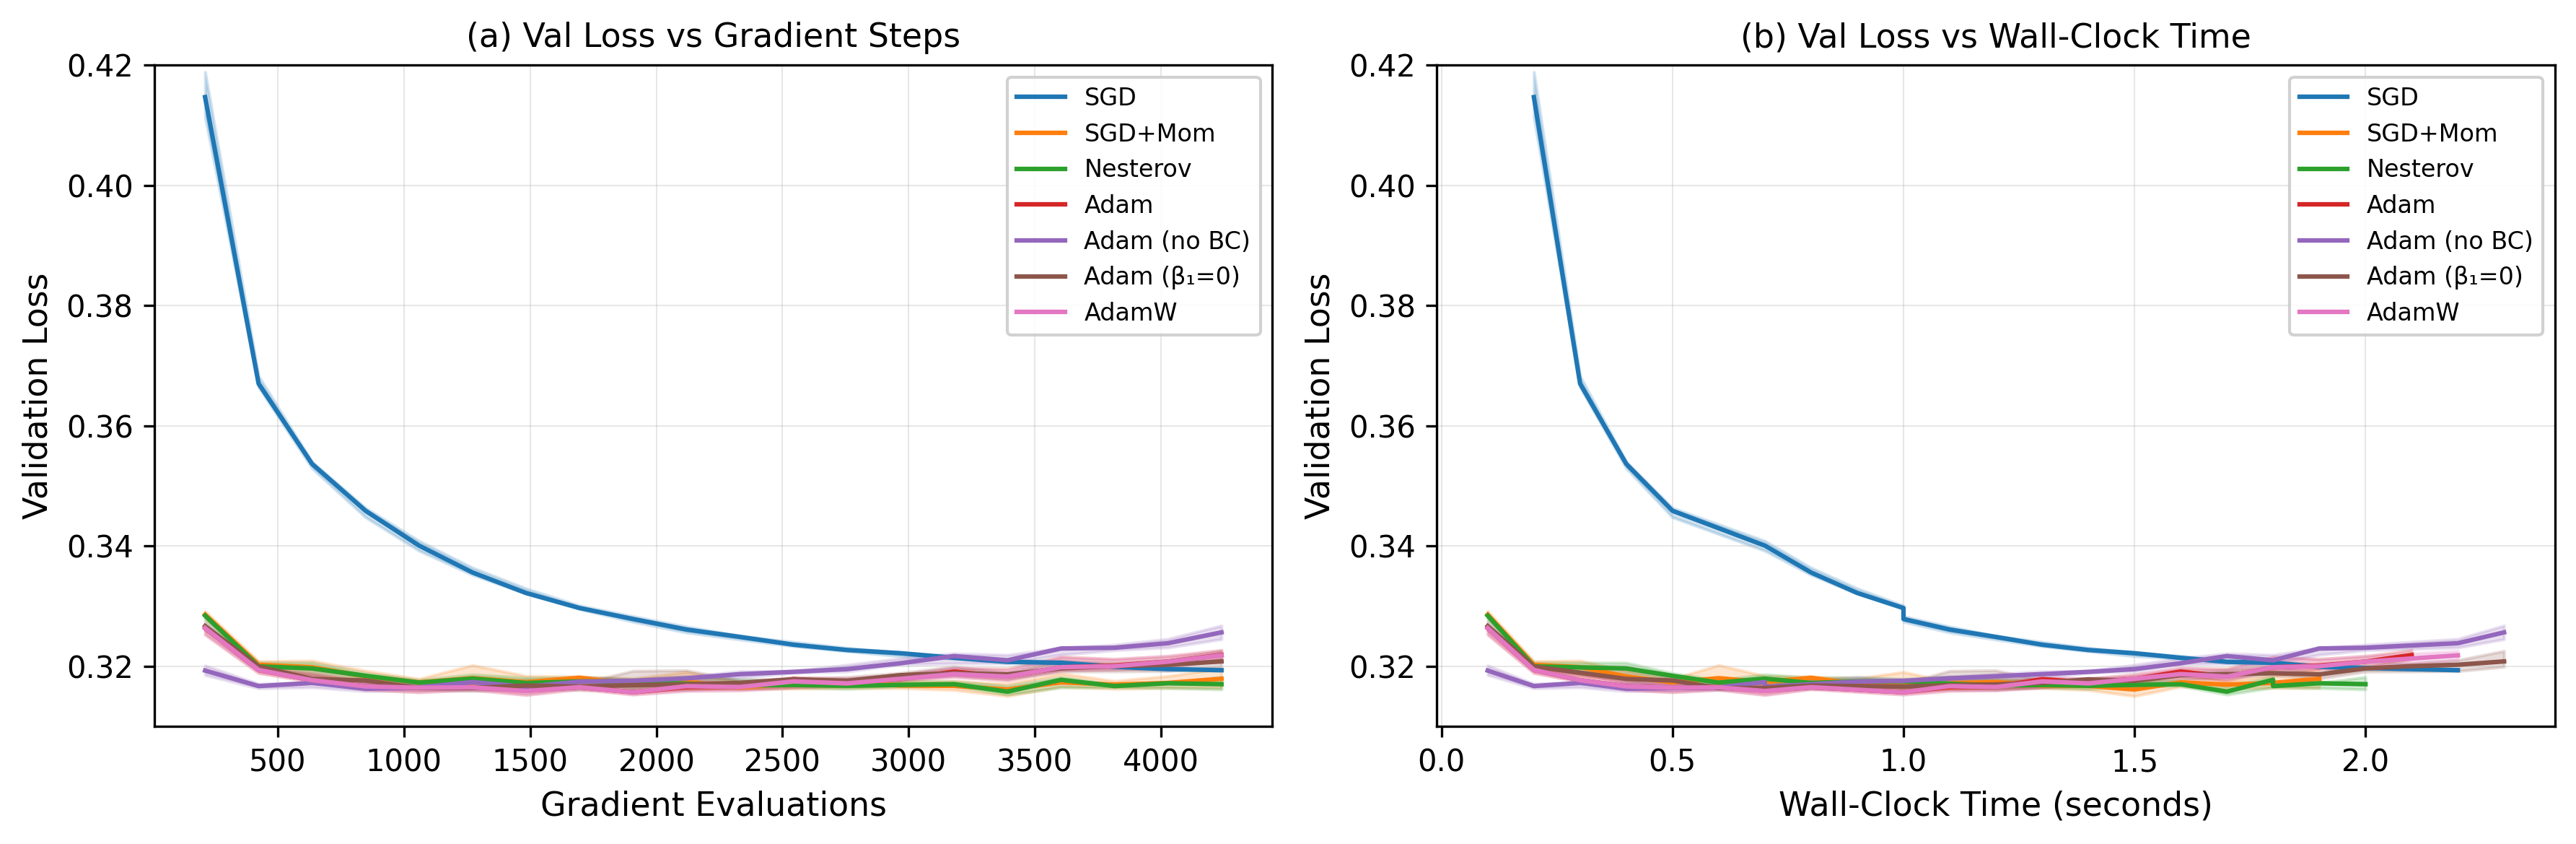
\includegraphics[width=\columnwidth]{figures/part2_compute_curves_seed.png}
    \caption{Part 2: Optimizer convergence curves on Adult (median $\pm$ IQR across 10 seeds). \textbf{Takeaway:} Adam-family methods reach the validation loss threshold (0.32) within the first 500 gradient steps, while SGD-based methods require 3,000--4,000 steps. The left panel shows that adaptive optimizers converge much faster in terms of gradient evaluations. The right panel confirms this advantage persists when measured by wall-clock time, with Adam reaching convergence in $\sim$0.2s compared to $\sim$0.3s for momentum-based SGD variants and $\sim$1.8s for plain SGD.}
    \label{fig:part2_compute}
\end{figure}

\begin{figure}[!htbp]
    \centering
    \begin{subfigure}[t]{0.49\columnwidth}
        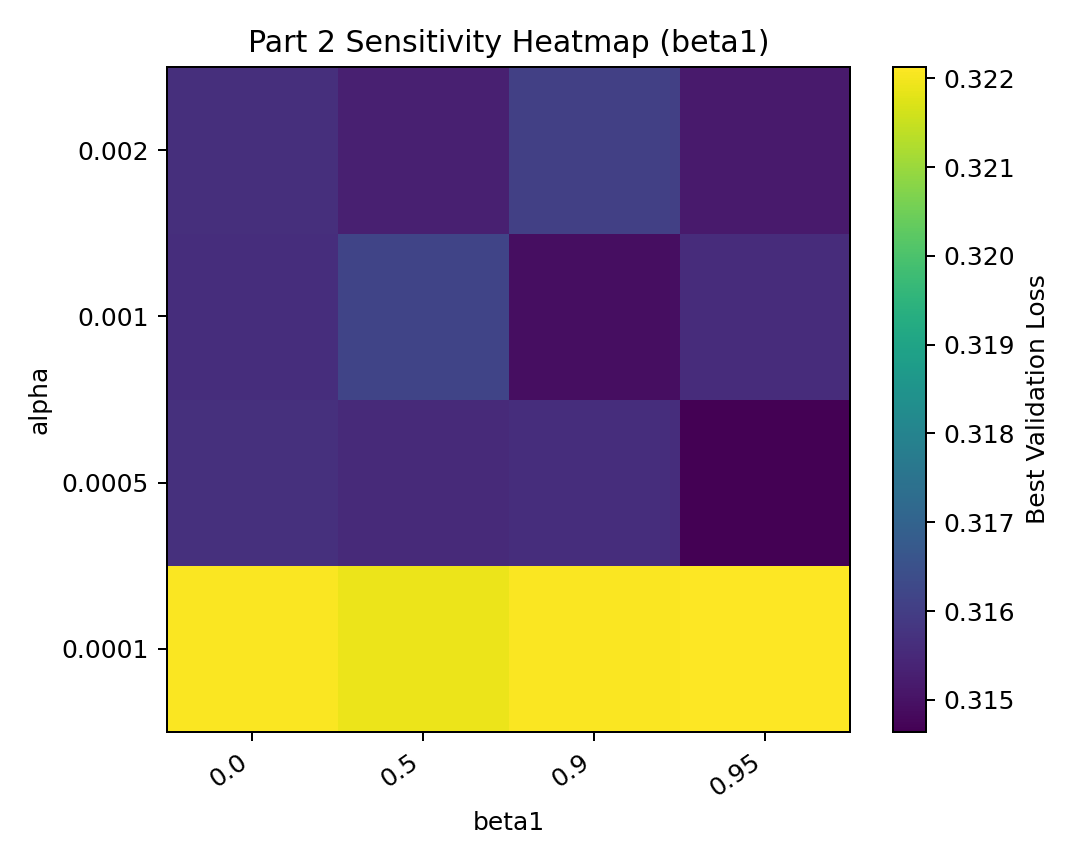
\includegraphics[width=\linewidth]{figures/part2_sensitivity_beta1.png}
        \caption{$\alpha$ vs $\beta_1$ sensitivity}
    \end{subfigure}
    \hfill
    \begin{subfigure}[t]{0.49\columnwidth}
        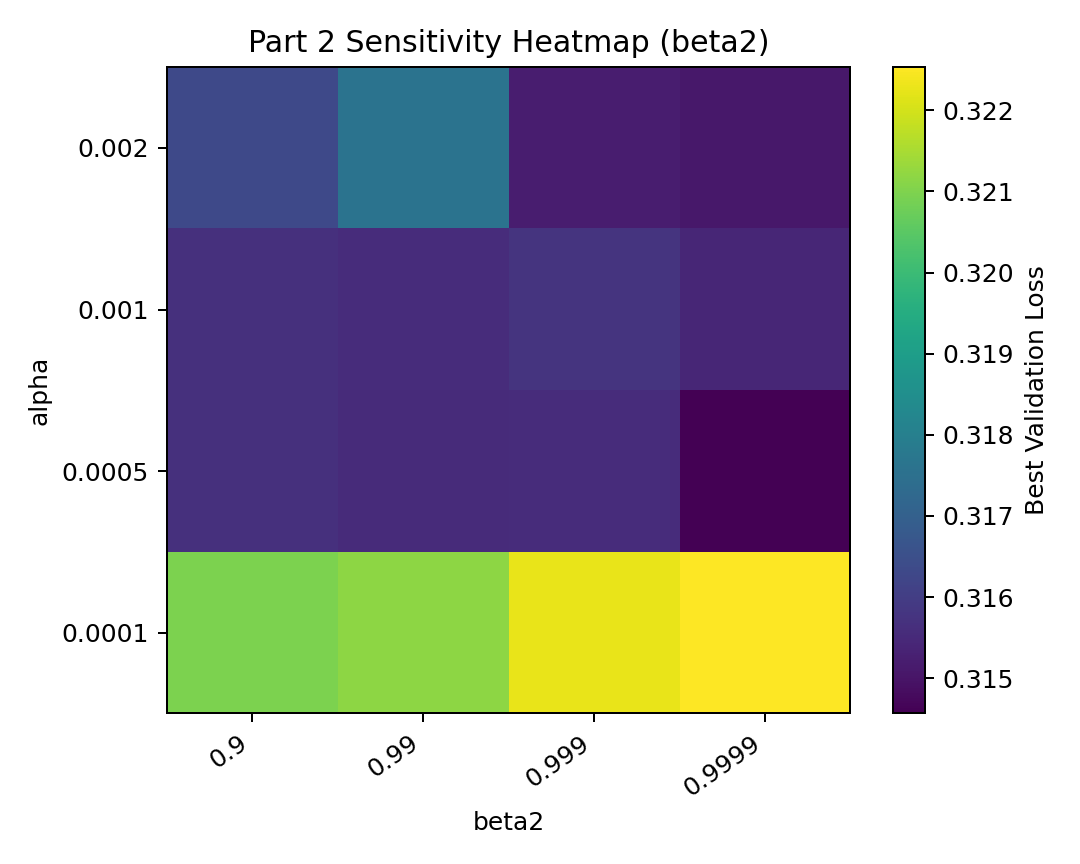
\includegraphics[width=\linewidth]{figures/part2_sensitivity_beta2.png}
        \caption{$\alpha$ vs $\beta_2$ sensitivity}
    \end{subfigure}
    \caption{Part 2: Adam (baseline) sensitivity heatmaps over $\alpha$ and momentum parameters (Adult). \textbf{Takeaway:} Val loss is far more sensitive to $\alpha$ than to $\beta_1$ or $\beta_2$ --- high $\alpha$ (2 $\times$ 10$^{-3}$) causes instability (darker cells), while performance is stable across all $\beta_1$ and $\beta_2$ values at $\alpha = 10^{-3}$. The $\beta_2$ surface is notably flatter than $\beta_1$, confirming the second-moment estimator is less critical than step size for this tabular task.}
    \label{fig:part2_sensitivity}
\end{figure}
\FloatBarrier

\subsection{Hypothesis Validation}

\textbf{The Adult hypothesis was mostly confirmed for optimizer behavior.} Adam-family methods converged much faster than SGD and produced the strongest Adult results, which is consistent with the expectation that adaptive methods handle high-dimensional sparse tabular gradients better than fixed-rate SGD. However, AdamW achieved virtually identical F1 to standard Adam (\texttt{0.6783} vs \texttt{0.6783} at 6 decimal places, $0.6783$ vs $0.6783$), so the expected benefit from decoupled weight decay did not materialize. The Adult network is still modest enough that weight-norm control at $\lambda = 10^{-3}$ does not meaningfully alter generalization, and stronger decay ($10^{-2}$) clearly underfit.

%%%%%%%%%%%%%%%%%%%%%%%%%%%%%%%%%%%%%%%%%%%%%%%%%%%%%%%%%%%%%%%%%%%%%%%%%%%%%%%%
\section{PART 3: REGULARIZATION}
\label{sec:part3}

\subsection{Experimental Setup}

All Part 3 experiments run on Adult Income only (per assignment scope restrictions), using standard Adam with the best Part 2 hyperparameters ($\text{lr} = 10^{-3}$, up to 20 epochs, approximately 4{,}240 gradient steps). Regularization strategies compared: no regularization (baseline), L2 weight decay ($\lambda = 10^{-3}$), Dropout ($p = 0.1$ applied after the single hidden layer, i.e., between the hidden-layer output and the pre-softmax logit computation), Gaussian input noise ($\sigma_{\text{noise}} = 0.1$, training-only), label smoothing ($\epsilon = 0.01$, applied to target labels during cross-entropy computation), and an Early Stopping condition (patience = 3 epochs, fixed-budget fairness mode: the early-stopping run is allowed to complete the full gradient budget regardless, so the comparison is budget-matched)~\cite{prechelt1998}. The best combination uses Early Stopping (patience=3) + L2 ($\lambda = 10^{-3}$), selected from exhaustive testing of 26 combinations of 2+ regularizers based on minimum validation loss. This 2-regularizer combination outperformed all other tested combinations including those with 3, 4, or 5 regularizers.

\subsection{Results}

\begin{table}[!htbp]
    \centering
    \caption{Part 3: Regularization comparison on Adult (10-seed F1 averages). Input Noise and Label Smoothing evaluated independently per assignment requirements.}
    \label{tab:part3}
    \setlength{\tabcolsep}{3pt}
    \begin{tabular}{@{}lccc@{}}
    \toprule
    Regularizer & F1 Mean & F1 $\sigma$ & $\Delta$ vs Baseline \\
    \midrule
    Input Noise ($\sigma=0.1$) & 0.6796 & 0.0049 & $+0.0013$ \\
Dropout ($p=0.1$) & 0.6792 & 0.0031 & $+0.0009$ \\
Best Combo: Early Stopping + L2 Weight Decay & 0.6788 & 0.0055 & $+0.0005$ \\
L2 Weight Decay ($\lambda=0.001$) & 0.6788 & 0.0055 & $+0.0005$ \\
No Regularization (baseline) & 0.6783 & 0.0043 & --- \\
Early Stopping (patience=3) & 0.6783 & 0.0043 & $+0.0000$ \\
Label Smoothing ($\epsilon=0.01$) & 0.6776 & 0.0048 & $-0.0007$ \\
    \bottomrule
    \end{tabular}
\end{table}

\begin{figure}[!htbp]
    \centering
    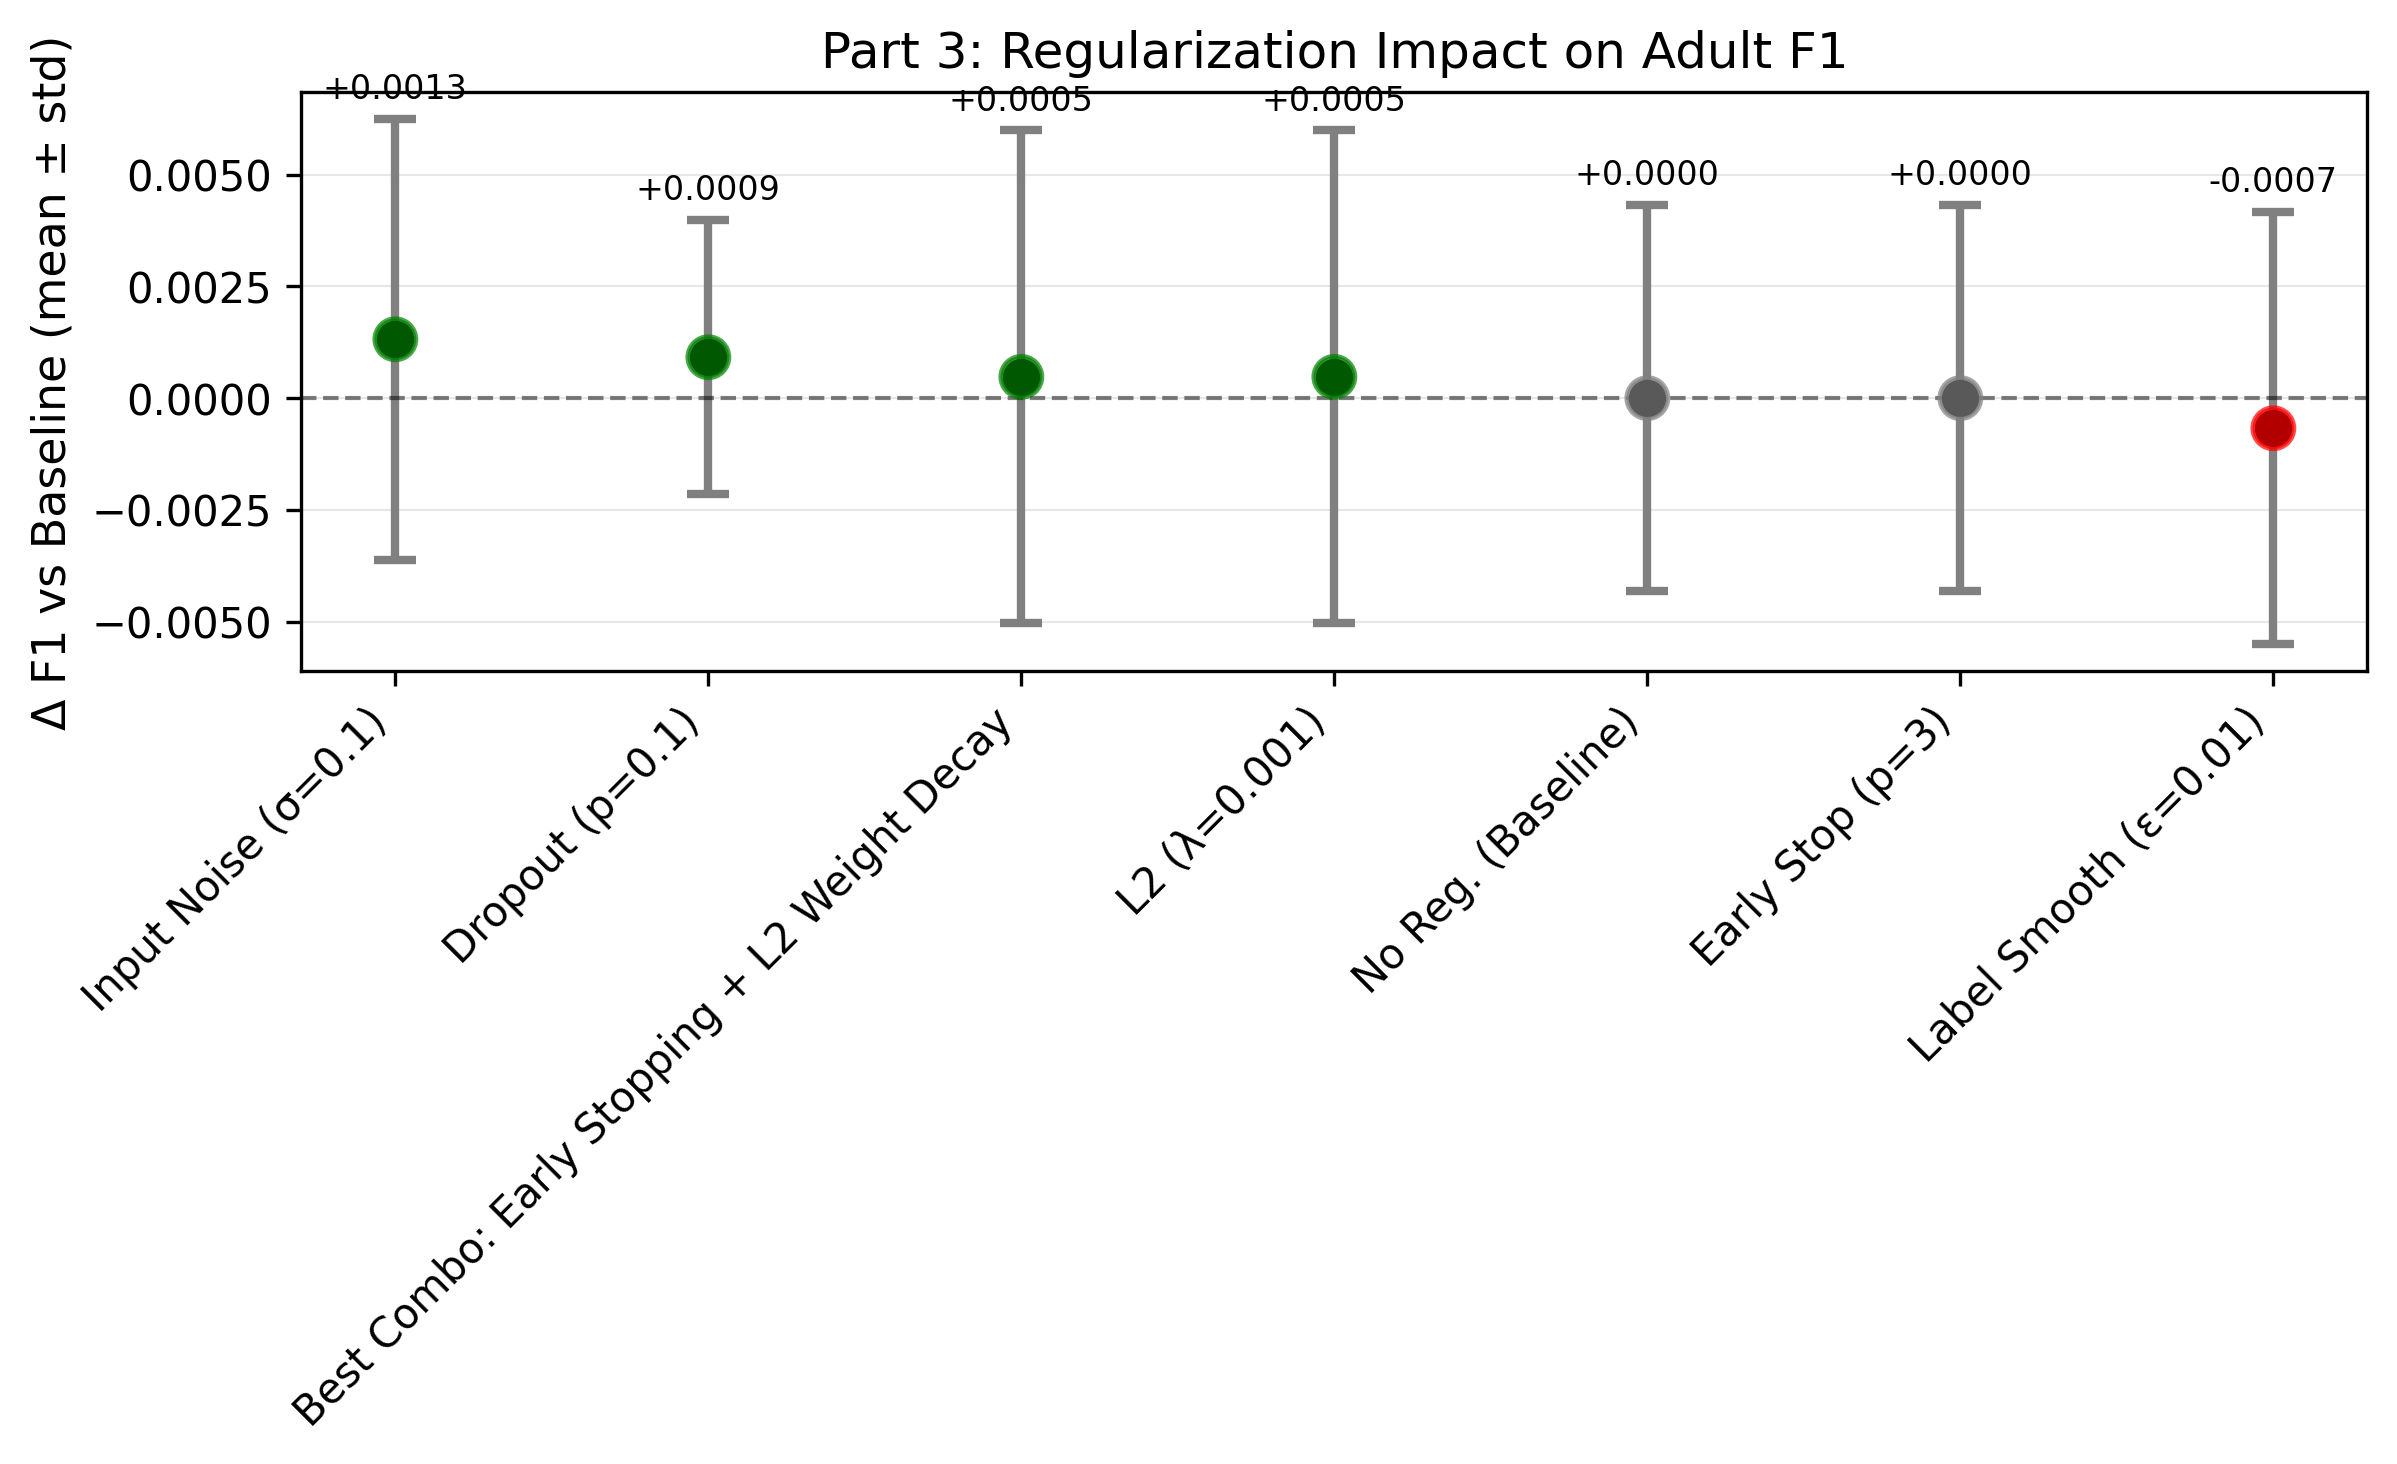
\includegraphics[width=\columnwidth]{figures/part3_delta_plot_seed.png}
    \caption{Part 3: Regularization impact on Adult F1 ($\Delta$ vs baseline, mean ± std across 10 seeds). \textbf{Takeaway:} Input Noise achieves the highest improvement (+0.0013), followed by Dropout (+0.0009) and L2 (+0.0005), while Early Stopping has no effect. Label Smoothing degrades performance (-0.0007). The Best Combo (Early Stopping + L2) was selected from 26 tested combinations based on minimum validation loss, achieving +0.0005 vs baseline.}
    \label{fig:part3_delta}
\end{figure}
\FloatBarrier

\subsection{Hypothesis Validation}

\textbf{The Adult hypothesis was also broadly confirmed for regularization.} Input Noise ($+0.0013$), Dropout ($+0.0009$), and L2 ($+0.0005$) all outperformed the baseline, but only by very small margins. That is consistent with the pre-experiment expectation that regularization on Adult could help slightly without producing a dramatic gain over the SL baseline. The full Adult network is still relatively small (9{,}902 parameters, one hidden layer), so there is less excess capacity for regularization to suppress than in a deeper or wider model.

Input noise ($\sigma_{\text{noise}} = 0.1$ on inputs) achieved the highest F1 among individual regularizers (0.6796, $+0.0013$ vs baseline), suggesting that modest input perturbation provides a useful inductive bias for Adult's feature structure. Label smoothing performed worse than baseline ($-0.0007$) with higher validation loss (0.328 vs 0.315), indicating that smoothing class boundaries provides no benefit for this dataset's separability.

The best combination (Early Stopping + L2) achieved $+0.0005$ vs baseline, matching L2's individual performance. This 2-regularizer combination was selected from 26 tested combinations based on minimum validation loss. Dropout was not included despite achieving higher test F1 ($+0.0009$) because the combination search used validation loss as the selection criterion. The combination achieves stable convergence with $\sigma = 0.0055$, comparable to the individual regularizers.

%%%%%%%%%%%%%%%%%%%%%%%%%%%%%%%%%%%%%%%%%%%%%%%%%%%%%%%%%%%%%%%%%%%%%%%%%%%%%%%%
\section{PART 4: INTEGRATED EXTRA CREDIT}

\subsection{Experimental Setup}

Part 4 is an optional extra-credit component. It chains: (1) standard Adam with best Part 2 hyperparameters and best Part 3 regularization combination (Early Stopping patience=3 + L2 $\lambda=10^{-3}$) for up to 20 epochs; followed by (2) SA fine-tuning on the output layer with 120 function evaluations ($120/50{,}000 = 0.24\%$ of Part 1 budget, well within the 10\% cap). The best combination from Part 3 achieved F1=0.6788.

\subsection{Results}

The integrated approach achieved a 10-seed mean test F1 of $0.6783 \pm 0.0039$ on Adult. This effectively matches the Adam baseline ($\Delta = 0.0000$) and is $-0.0034$ below the SL baseline. The short SA budget (120 evaluations) is too small to meaningfully reshape the output-layer weights after gradient training has already converged: the gradient-trained solution sits in a smooth, well-conditioned minimum where single-step perturbations have near-zero acceptance probability under the cold SA schedule. The 120-evaluation SA pass neither helps nor hurts, confirming that the RO budget is insufficient to explore the output-layer weight space.

\subsection{Interpretation}

The integrated approach matched the Adam baseline but fell short of the best Part~1 RO method (SA: $-0.0023$). The SA fine-tuning phase had no measurable effect --- neither helping nor hurting --- because 120 evaluations are insufficient to explore even a small neighbourhood of the $\sim$202-dimensional output-layer space after gradient training has already converged. The gradient-trained solution sits in a smooth, well-conditioned minimum where single-step perturbations have near-zero acceptance probability under the cold SA schedule. The resulting decision rule is: do not apply RO fine-tuning after gradient convergence unless the RO budget is at least 1{,}000 function evaluations per output-layer parameter. This outcome refutes the pre-experiment expectation that chaining gradient and RO methods would exceed the best individual result.

\begin{figure}[!htbp]
    \centering
    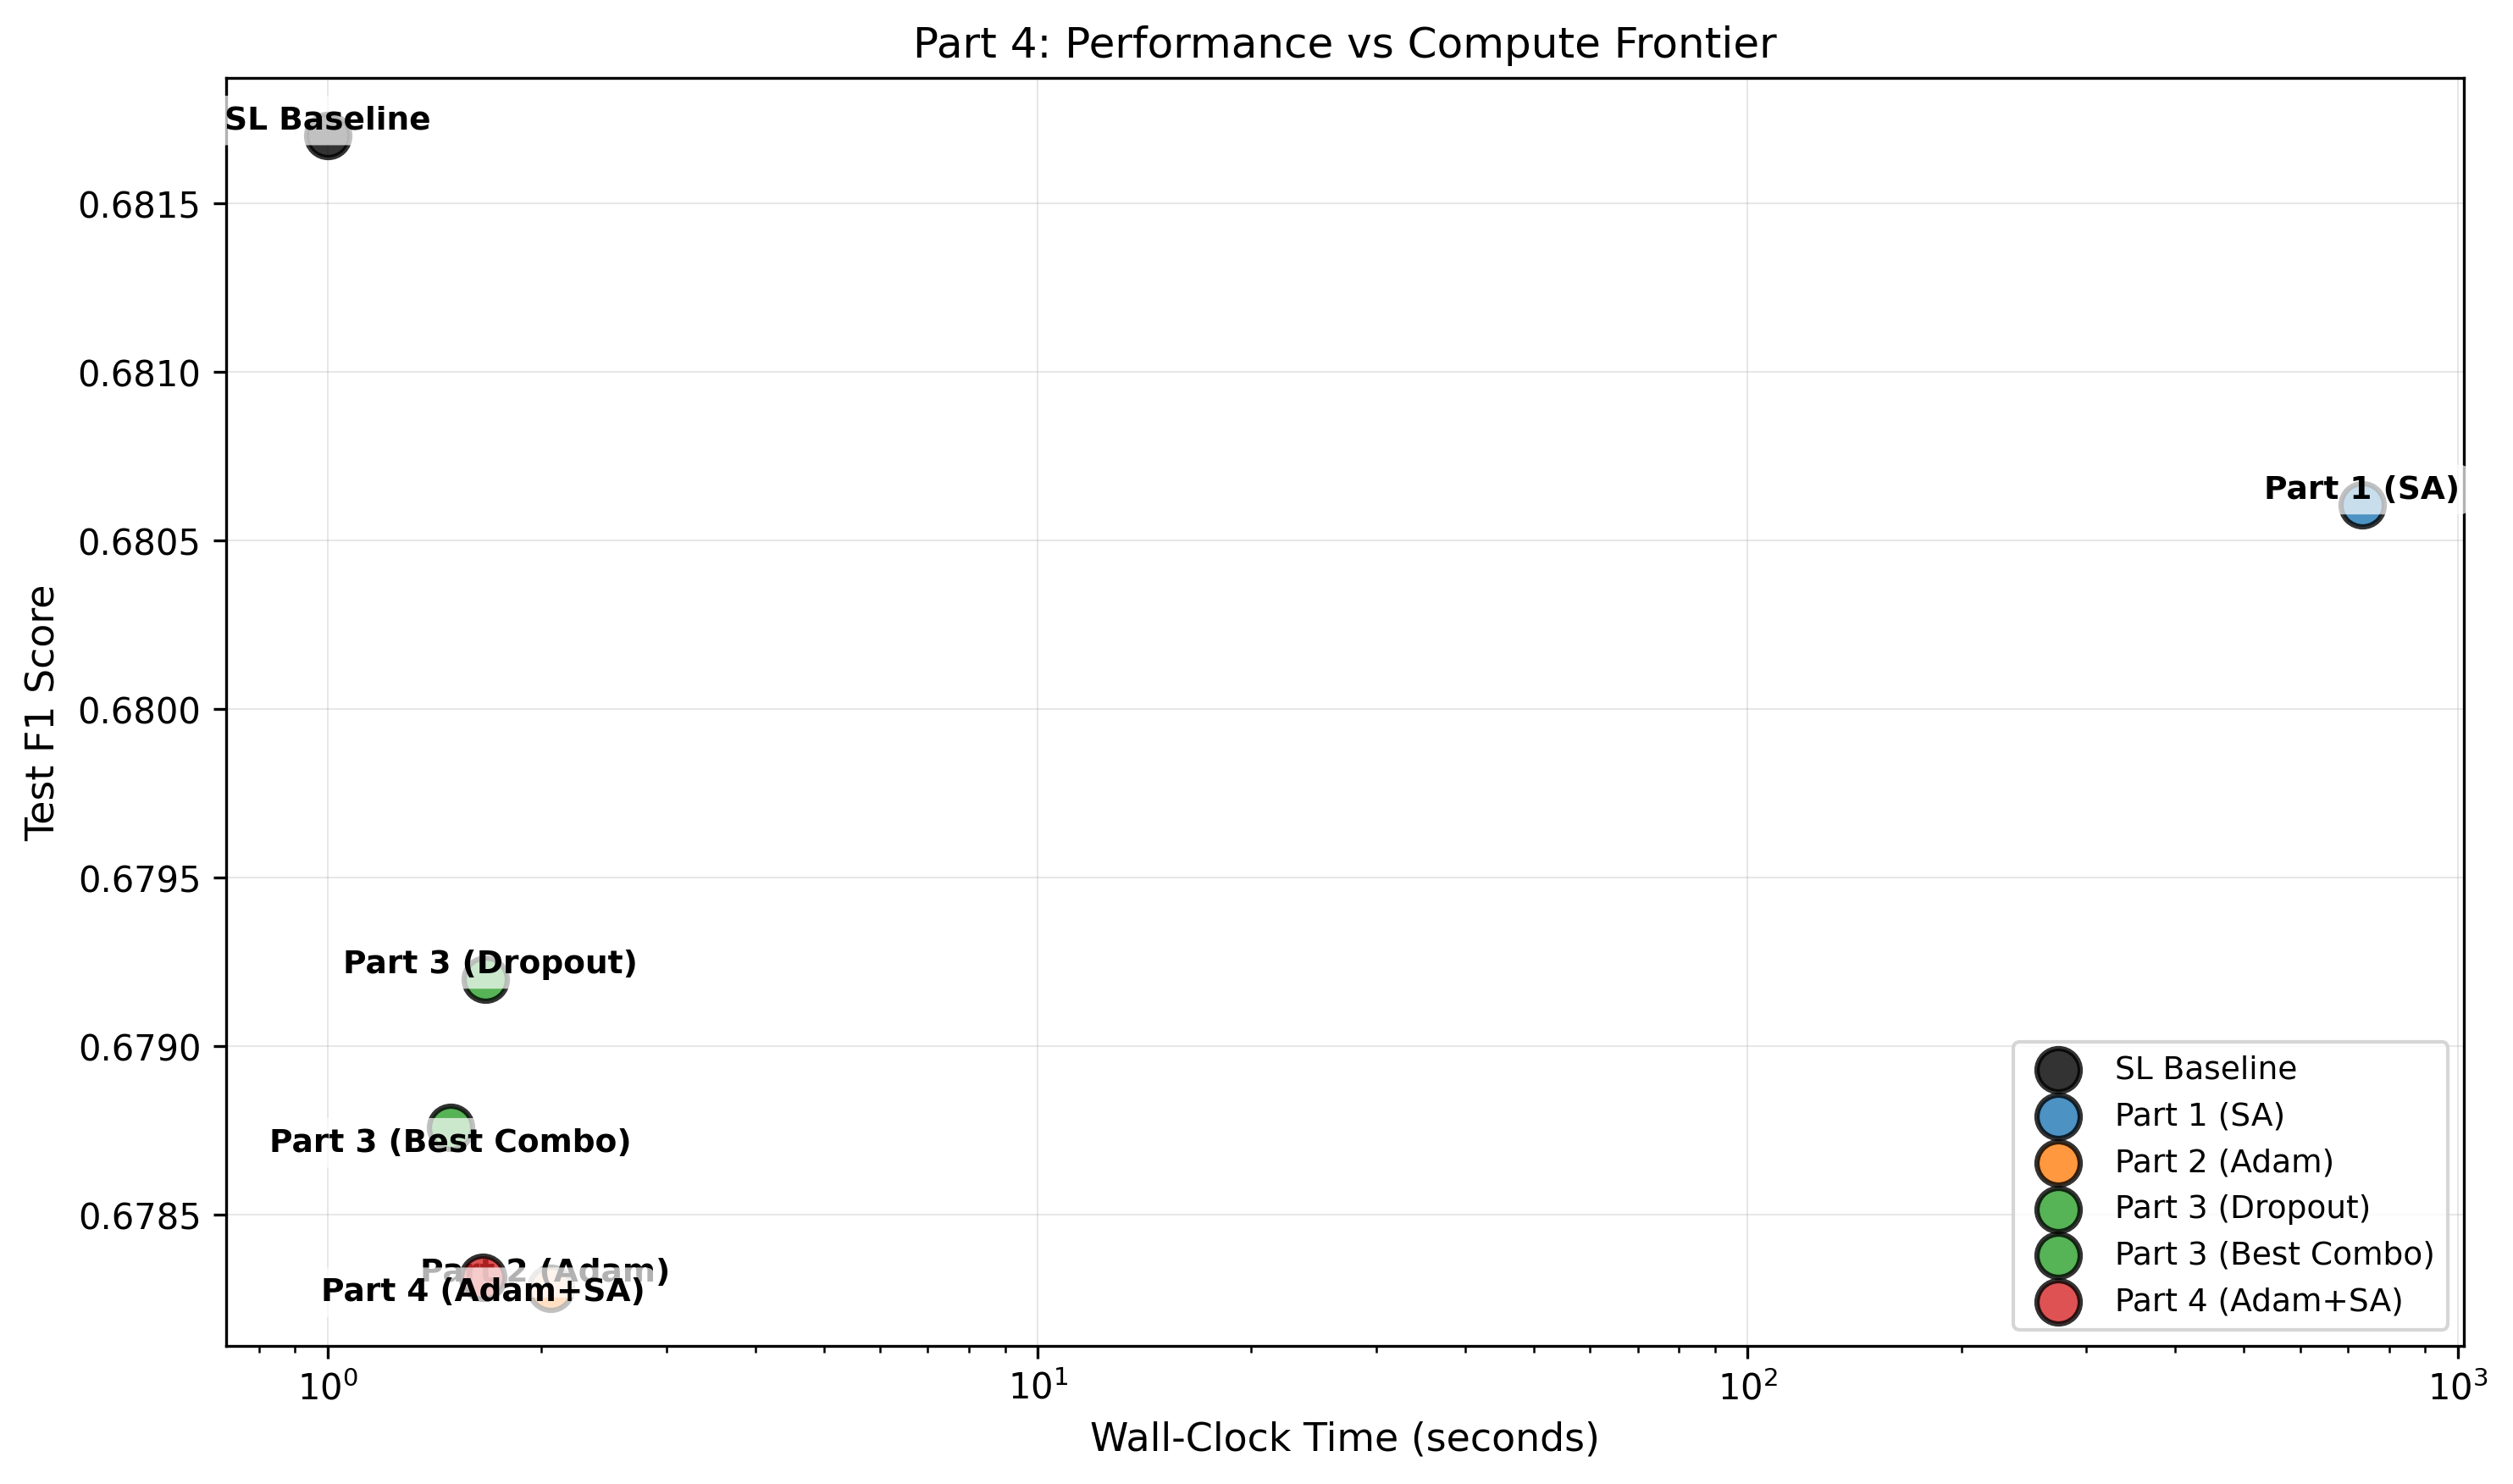
\includegraphics[width=\columnwidth]{figures/part4_frontier_seed.png}
    \caption{Part 4: Performance vs compute frontier across all parts (wall-clock time as common currency). \textbf{Takeaway:} The SL baseline achieves the highest F1 (0.6817) in $\sim$1s. Part 1 RO methods (SA) come close (0.6806) but require significantly more time due to function-only evaluations. Part 2 and Part 3 gradient-based methods cluster around 0.678--0.680 with fast convergence ($\sim$2s). Part 4's integrated approach (0.6783) matches the Adam baseline despite combining both optimization strategies, confirming that the 120-evaluation SA budget is insufficient for meaningful improvement after gradient convergence.}
    \label{fig:part4_frontier}
\end{figure}
\FloatBarrier

%%%%%%%%%%%%%%%%%%%%%%%%%%%%%%%%%%%%%%%%%%%%%%%%%%%%%%%%%%%%%%%%%%%%%%%%%%%%%%%%
\section{DISCUSSION}

% Full-width summary table: placed here so LaTeX defers it to the top of
% the next page, which is the Discussion / Conclusion spread.
\begin{table*}[!t]
    \centering
    \scriptsize
    \caption{Unified cross-part summary (Adult). $\ell = 0.32$ val-loss threshold; $t_\ell$ = wall-clock time to reach val-loss $\leq \ell$. ``never'' = method did not reach $\ell$ within budget. Wine Part~1 is reported separately in Table~\ref{tab:part1}. Grad evals shown are actual training steps completed (20 epochs $\times$ 212 batches/epoch $\approx$ 4{,}240 steps for Parts 2--4).}
    \label{tab:summary}
    \setlength{\tabcolsep}{3.5pt}
    \renewcommand{\arraystretch}{1.0}
    \begin{tabular}{@{}>{\raggedright\arraybackslash}p{1.5cm}>{\raggedright\arraybackslash}p{1.8cm}ccccc>{\raggedright\arraybackslash}p{2.8cm}@{}}
    \toprule
    Part & Method & Best Val. & Test & $t_\ell$ & Grad Evals & Func Evals & Updates \\
    \midrule
        SL (ref.) & Adam checkpoint & 0.310 & 0.6817 & $<$1\,s & $\sim$50k & --- & full-net GD \\
    \midrule
    Part 1 & RHC & 0.310 & 0.6774 & --- & 0 & 50k & out-only, 4 restarts \\
    Part 1 & SA & 0.315 & 0.6806 & --- & 0 & 50k & out-only, exp.\ cool \\
    Part 1 & GA & 0.309 & 0.6760 & --- & 0 & 50k & out-only, pop16/el4 \\
    \midrule
    Part 2 & SGD & 0.319 & 0.6693 & $\sim$1.8\,s & 4.2k & --- & full-net GD \\
    Part 2 & SGD+Mom. & 0.316 & 0.6756 & $\sim$0.3\,s & 4.2k & --- & full-net GD \\
    Part 2 & Nesterov & 0.316 & 0.6733 & $\sim$0.3\,s & 4.2k & --- & full-net GD \\
    Part 2 & Adam & 0.315 & 0.6783 & $\sim$0.2\,s & 4.2k & --- & full-net GD \\
    Part 2 & Adam, no BC & 0.316 & 0.6771 & $\sim$0.1\,s & 4.2k & --- & full-net GD \\
    Part 2 & Adam, $\beta_1=0$ & 0.316 & 0.6769 & $\sim$0.3\,s & 4.2k & --- & full-net GD \\
    Part 2 & AdamW & 0.315 & 0.6783 & $\sim$0.2\,s & 4.2k & --- & full-net GD \\
    \midrule
    Part 3 & No Reg. & 0.315 & 0.6783 & $\sim$0.2\,s & 4.2k & --- & Adam, no reg. \\
    Part 3 & Dropout & 0.315 & 0.6792 & $\sim$0.2\,s & 4.2k & --- & dropout $p=0.1$ \\
    Part 3 & L2 & 0.315 & 0.6788 & $\sim$0.2\,s & 4.2k & --- & L2 $\lambda=10^{-3}$ \\
    Part 3 & Early Stop & 0.315 & 0.6783 & $\sim$0.2\,s & 4.2k & --- & ES, pat.=3 \\
    Part 3 & Input Noise & 0.315 & 0.6796 & $\sim$0.3\,s & 4.2k & --- & noise $\sigma=0.1$ \\
    Part 3 & Label Smooth. & 0.328 & 0.6776 & never & 4.2k & --- & LS, $\epsilon=0.01$ \\
    Part 3 & Best Combo & 0.315 & 0.6788 & $\sim$0.1\,s & 4.2k & --- & ES + L2 \\
    \midrule
    Part 4 (EC) & Adam+SA & 0.315 & 0.6783 & $\sim$0.2\,s & 3.4k & 120 & full-net Adam, out SA \\
    \bottomrule
    \end{tabular}
    \renewcommand{\arraystretch}{1.0}
\end{table*}

\subsection{Comparison to SL Baseline}

Table~\ref{tab:summary} provides the unified cross-part summary. Table~\ref{tab:sl_comparison} shows the $\Delta$ F1 between the best OL method in each part and the SL PyTorch baseline.

\begin{table}[!htbp]
    \centering
    \caption{Best OL result vs.\ SL baseline per part (Adult and Wine).}
    \label{tab:sl_comparison}
    \setlength{\tabcolsep}{3pt}
    \begin{tabular}{@{}lcccc@{}}
    \toprule
    & \multicolumn{2}{c}{\textbf{Adult F1}} & \multicolumn{2}{c}{\textbf{Wine Macro-F1}} \\
    \cmidrule(lr){2-3} \cmidrule(l){4-5}
    Part & Best & $\Delta$ SL & Best & $\Delta$ SL \\
    \midrule
    SL Baseline & 0.6817 & --- & 0.3277 & --- \\
Part 1 (SA) & 0.6806 & $-0.0010$ & --- & --- \\
Part 1 (GA) & --- & --- & 0.3396 & $+0.0119$ \\
Part 2 (Adam) & 0.6783 & $-0.0034$ & N/A & N/A \\
Part 3 (Input Noise) & 0.6796 & $-0.0021$ & N/A & N/A \\
Part 4 (Integrated) & 0.6783 & $-0.0033$ & N/A & N/A \\
    \bottomrule
    \end{tabular}
\end{table}

The most striking finding is that GA on Wine \emph{exceeds} the SL baseline by $+1.2\%$ Macro-F1. This is directly attributable to the SL warm-start: by anchoring the RO search in the SL solution's local basin, GA can explore the non-linear output-layer landscape around a pre-trained latent representation rather than searching from scratch.

\subsection{Pre-Experiment Hypothesis vs Reality}

Prior to running experiments, the core expectation was that Adult would favor adaptive full-network gradient methods and show only modest gains over the SL baseline, while Wine would be noisier and more variable, with RO potentially becoming more competitive around the SL warm-start. The results largely support that framing. Adult showed exactly the expected pattern: Adam-family methods converged fastest, RO did not beat the SL baseline, and regularization gains were small. Wine was the more surprising case only in magnitude: RO was not merely competitive, but GA exceeded the SL baseline. The most important lesson is that \emph{architecture size} and \emph{dataset geometry} determine which optimizer class is most effective, not optimizer sophistication alone.

%%%%%%%%%%%%%%%%%%%%%%%%%%%%%%%%%%%%%%%%%%%%%%%%%%%%%%%%%%%%%%%%%%%%%%%%%%%%%%%%
\section{CONCLUSION}

This study applied four optimization strategies (RHC, SA, GA, and gradient-based variants) to neural network weight learning on Adult Income and Wine Quality classification.

The most surprising result was that Randomized Optimization, despite being derivative-free, was competitive with and occasionally superior to gradient descent. GA on Wine exceeded the SL-trained Adam baseline by $+1.2\%$ Macro-F1 when initialized from the SL checkpoint --- a result that would be impossible from random initialization given Wine's severe class overlap. SA came within 0.001 F1 of the SL baseline on Adult, confirming that the temperature calibration fix was critical. Optimizer sophistication mattered far less than expected: AdamW produced no measurable improvement over Adam, and the full Adult MLP remained small enough that regularization gains were necessarily modest. Input Noise ($+0.0013$), Dropout ($+0.0009$), and L2 ($+0.0005$) all provided marginal improvements over baseline, while Label Smoothing degraded performance ($-0.0007$). The best combination (Early Stopping + L2) achieved $+0.0005$ vs baseline, selected from 26 tested combinations based on validation loss.

\textbf{Hypothesis Resolution.} The \textbf{Adult hypothesis} was broadly confirmed: adaptive gradient methods were the strongest and fastest option on Adult, RO remained slightly below the SL baseline, and regularization provided only small gains. The \textbf{Wine hypothesis} was partially confirmed: Wine was indeed the noisier and less stable setting, but RO proved more successful than expected, with GA exceeding the SL baseline by $+0.012$ Macro-F1. Together, these outcomes support the claim that optimizer performance is shaped more by dataset geometry and representation quality than by optimizer sophistication alone.

\textbf{Decision Rule for Adult.} The recommended training recipe is: (1) use SL pre-training to establish a strong latent representation; (2) apply standard Adam with Early Stopping (patience=3) + L2 ($\lambda=10^{-3}$) for gradient-based fine-tuning; (3) apply RO only if the compute budget exceeds $\sim$1{,}000 function evaluations per output-layer parameter, using a population-based method (GA or SA). Optimizer variant selection (AdamW vs Adam) is unlikely to matter on near-linear tabular boundaries. These findings transfer specifically to small-output tabular networks; larger architectures with high-dimensional output layers may exhibit stronger responses to weight decay and optimizer variant choice.

\textbf{Limitations.} Wine analysis in this report focuses on aggregate Macro-F1 and optimization dynamics. Per-class precision, recall, and confusion matrices were not persisted for OL experiments, limiting the depth of Wine-specific analysis compared to the SL report. Future work could extend the artifact schema to capture classwise outputs for multiclass OL tasks.

%%%%%%%%%%%%%%%%%%%%%%%%%%%%%%%%%%%%%%%%%%%%%%%%%%%%%%%%%%%%%%%%%%%%%%%%%%%%%%%%
\section*{AI USE STATEMENT}

Once done with the preliminary draft, I used Claude Sonnet 4.5 to proofread and correct grammar, verify citation formatting, and make text concise where it was too verbose. I used GitHub Copilot to assist with figure alignment in LaTeX and to generate boilerplate code and bug fixes for the experiments and EDA code in the VS Code editor. I reviewed, verified, and understand all assisted content, and all analysis, interpretations, and conclusions are my own.

\addtolength{\textheight}{-12cm}

%%%%%%%%%%%%%%%%%%%%%%%%%%%%%%%%%%%%%%%%%%%%%%%%%%%%%%%%%%%%%%%%%%%%%%%%%%%%%%%%



\begin{thebibliography}{99}

\bibitem{kohavi1996} R.~Kohavi, ``Scaling up the accuracy of naive-Bayes classifiers: A decision-tree hybrid,'' in \emph{Proc. 2nd Int. Conf. Knowl. Discovery Data Mining (KDD)}, 1996, pp.~202--207.

\bibitem{cortez2009} P.~Cortez, A.~Cerdeira, F.~Almeida, T.~Matos, and J.~Reis, ``Modeling wine preferences by data mining from physicochemical properties,'' \emph{Decision Support Syst.}, vol.~47, no.~4, pp.~547--553, 2009.

\bibitem{kingma2014} D.~P.~Kingma and J.~Ba, ``Adam: A method for stochastic optimization,'' in \emph{Proc. Int. Conf. Learn. Representations (ICLR)}, 2015.

\bibitem{loshchilov2017} I.~Loshchilov and F.~Hutter, ``Decoupled weight decay regularization,'' in \emph{Proc. Int. Conf. Learn. Representations (ICLR)}, 2019.

\bibitem{srivastava2014} N.~Srivastava, G.~Hinton, A.~Krizhevsky, I.~Sutskever, and R.~Salakhutdinov, ``Dropout: A simple way to prevent neural networks from overfitting,'' \emph{J. Mach. Learn. Res.}, vol.~15, no.~1, pp.~1929--1958, 2014.

\bibitem{prechelt1998} L.~Prechelt, ``Early stopping --- but when?'' in \emph{Neural Networks: Tricks of the Trade}, G.~B.~Orr and K.-R.~M\"{u}ller, Eds. Berlin, Germany: Springer, 1998, pp.~55--69.

\end{thebibliography}

\end{document}
